\begin{center}
  \Large
  \textbf{BIOGRAFI PENULIS}
\end{center}

\addcontentsline{toc}{chapter}{BIOGRAFI PENULIS}

\vspace{2ex}

\begin{wrapfigure}{L}{0.3\textwidth}
  \centering
  \vspace{-3ex}
  % Ubah file gambar berikut dengan file foto dari mahasiswa
  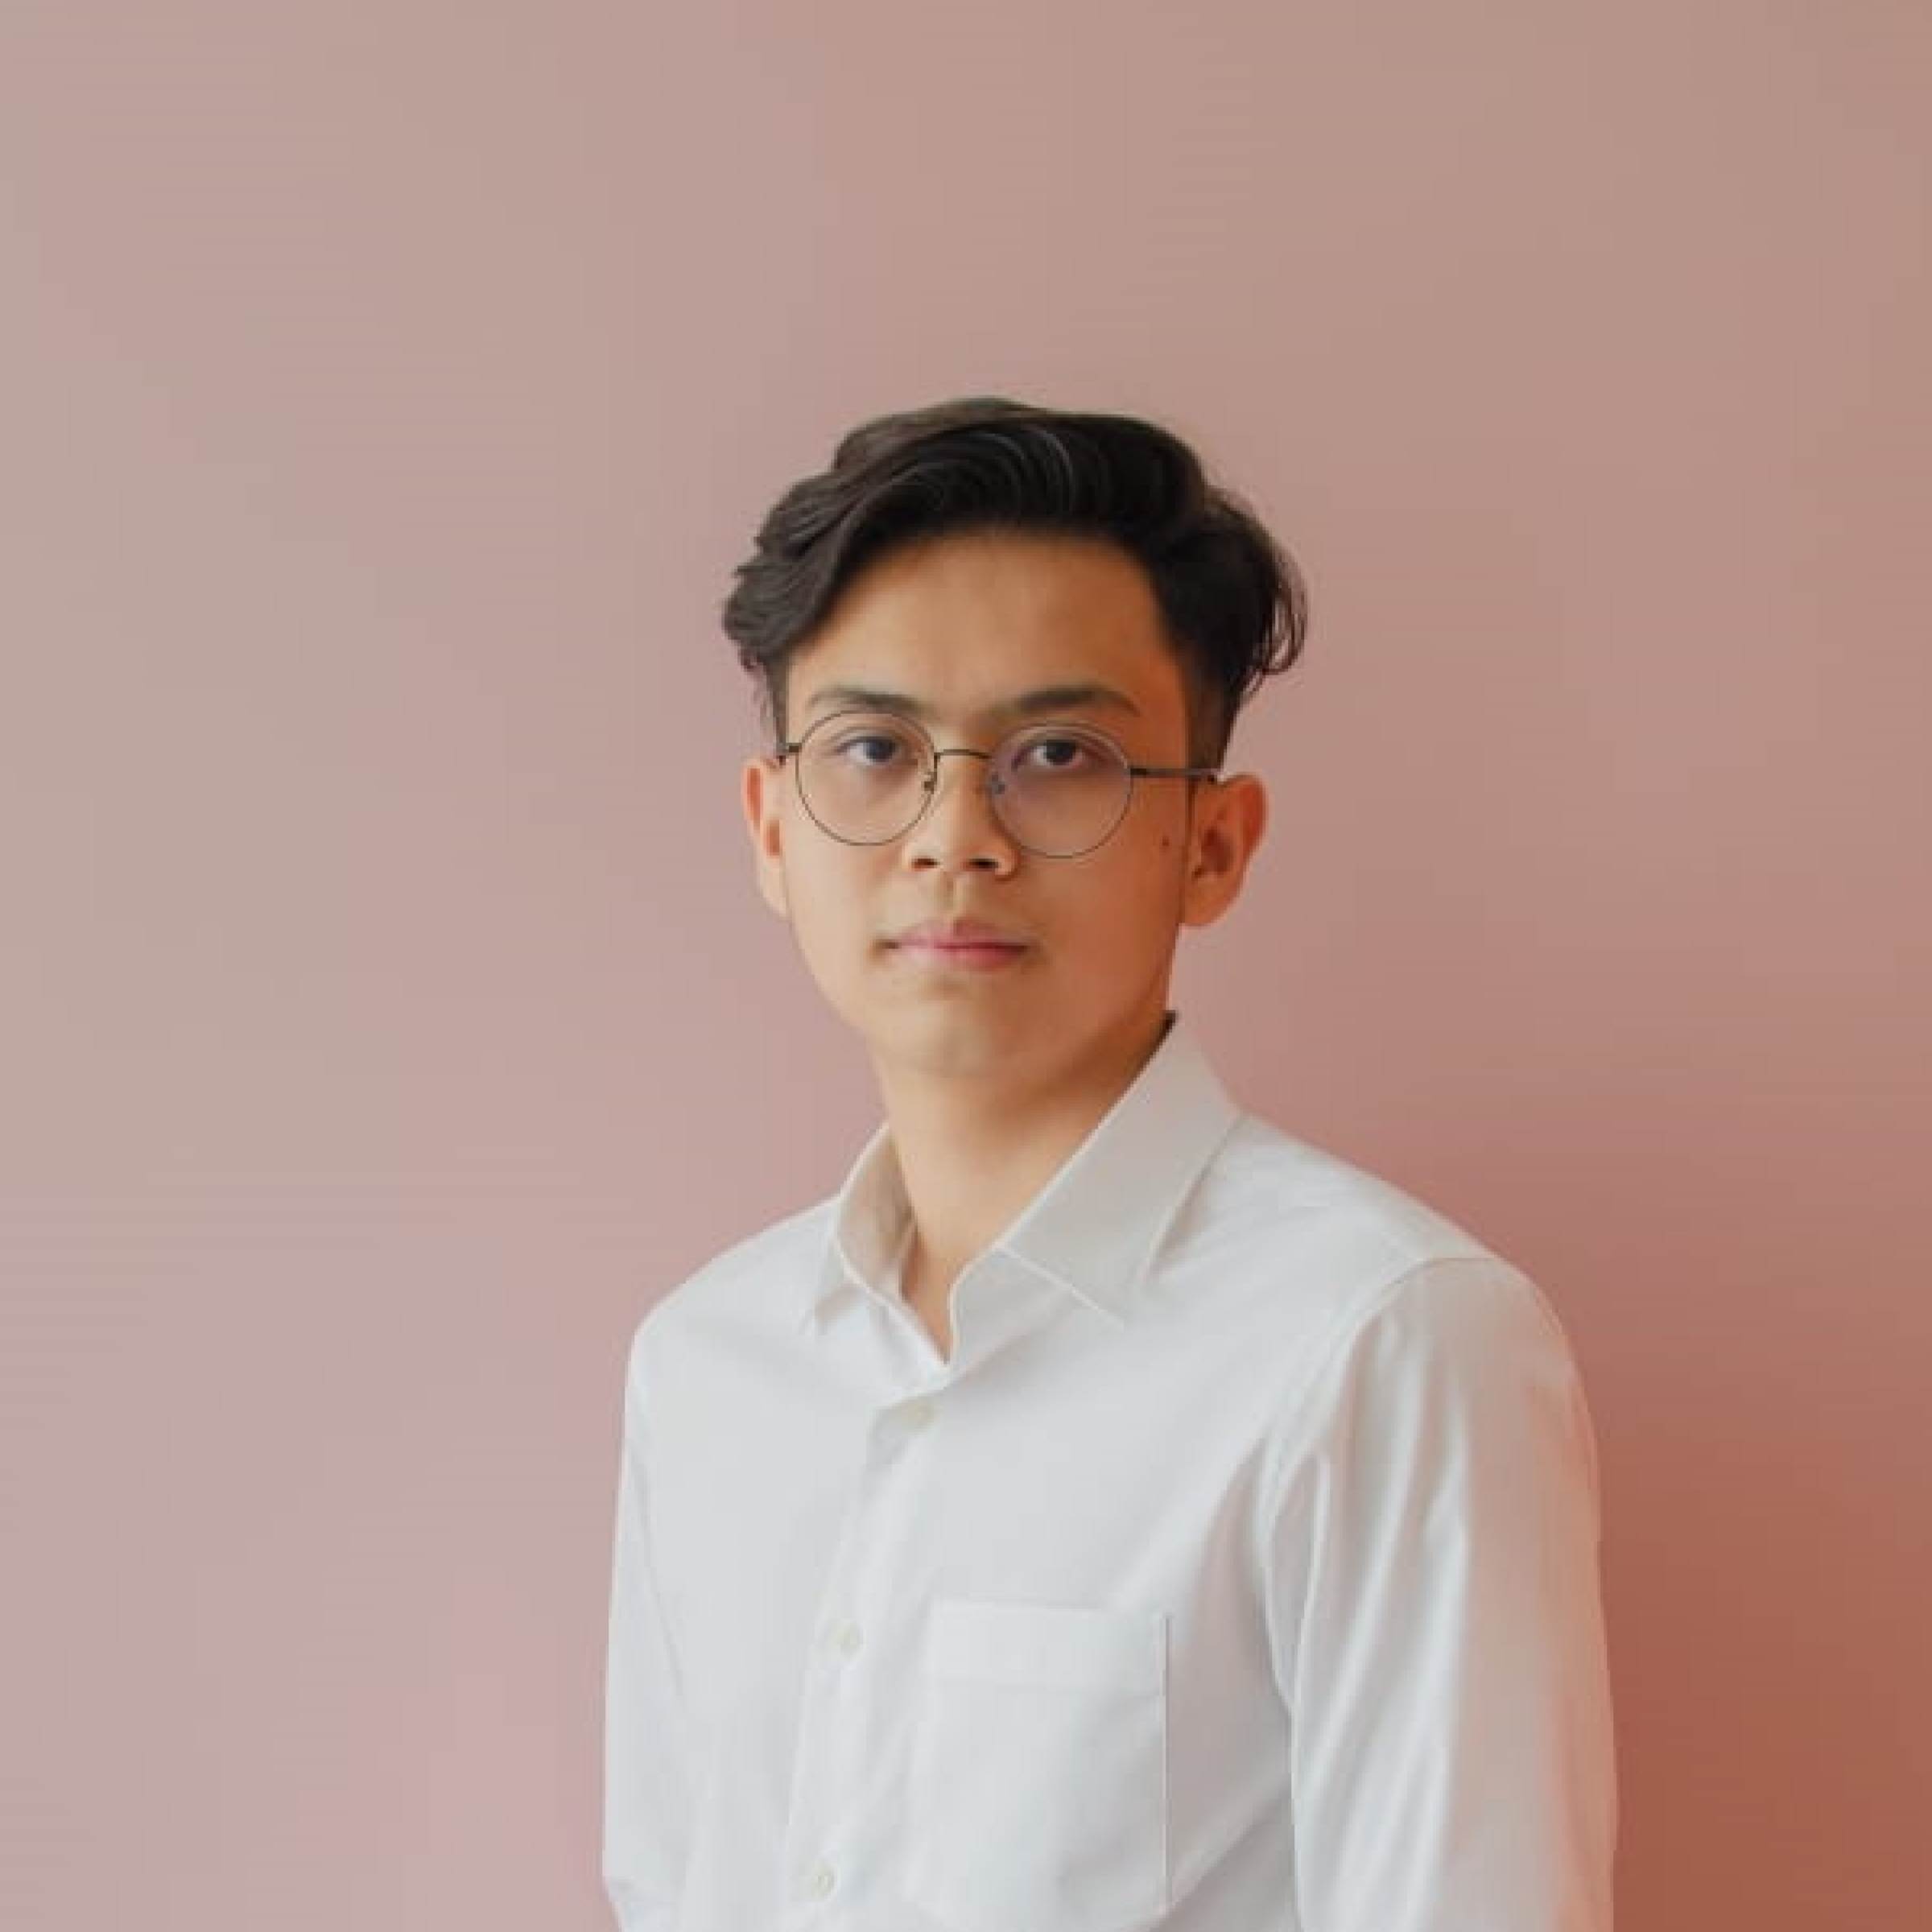
\includegraphics[width=0.3\textwidth]{gambar/foto-formal.png}
  \vspace{-4ex}
\end{wrapfigure}

% Ubah kalimat berikut dengan biografi dari mahasiswa
\name{}, atau yang biasa dikenal sebagai Krisna, lahir di Gianyar, Bali pada 8 Juli 2002. Penulis merupakan anak pertama dari tiga bersaudara yang tinggal dan tumbuh besar di Kota Denpasar, Bali. Ketertarikan mendalam penulis di bidang teknologi mengantarkan penulis yang telah menyelesaikan masa sekolah di SMA Negeri 4 Denpasar ke jenjang strata satu di Departemen Teknik Komputer Fakultas Teknologi Elektro dan Informatika Cerdas Institut Teknologi Sepuluh Nopember (ITS) pada tahun 2020.

Penulis merupakan pribadi yang memiliki ketertarikan dalam menjelajahi topik - topik yang berkaitan dengan bidang teknologi secara tekun dan mendalam. Dalam masa kuliah, penulis tertarik dengan topik seperti \emph{Internet Of Things} (IOT), Pengembangan Aplikasi (\emph{Mobile Development}), \emph{Machine Learning}, dan \emph{Computer Vision}. Penulis juga aktif dalam mengembangkan minat dan bakat di luar perkuliahan. Hal ini dibuktikan dengan rekam jejak organisasi dan kepanitian dari penulis seperti Wakil Ketua I Multimedia and Game Development (MAGE) 8, Koordinator Asisten Laboratorium Multimedia dan \emph{Internet Of Things} (IOT), hingga mengikuti program Bangkit Academy 2023. Hingga saat ini penulis terus menekani ketertarikan dan kemampuan yang dimiliki di bidang teknologi, terkhususnya pada bidang Pengembangan Aplikasi (\emph{Mobile Development}) dan \emph{Computer Vision}.

Pada penelitian tugas akhir ini, penulis memilih mengembangkan sistem penerjemah bahasa isyarat Indonesia (BISINDO) yang berfokus pada bidang \emph{Computer Vision}. Keresahan penulis yang memiliki suadara perempuan yang mengalami keterbatasan pendengaran dan berkomunikasi dengan bahasa isyarat menginspirasi dibuatnya tugas akhir ini sebagai bentuk upaya dalam memudahkan komunikasi teman tuli dengan khalayak umum. Bagi pembaca yang memiliki kritik, saran, atau pertanyaan mengenai tugas akhri ini dapat menghubungi penulis melalui surel krisnaerlangga08@gmail.com.
